\chapter{Implementation}
Now that the analysis of the conversion and the converter design is complete, it is time to consider the converter's implementation. A substantial part of the converter system can be implemented by simply creating a java structure corresponding to the conceptual structure given in the design section. For example, a converter component could be realized as a package containing classes and interfaces, which define its sub-components. The tasks performed by each of these components could then be implemented as methods in the corresponding classes, according to the conversion rules specified in the analysis. However, when it comes to implementations there are often multiple ways to achieve the same goals and sometimes practical limitations that can prevent you from using a certain approach. 

In this section, some of the most prominent implementation choices will be showcased to give an understanding how the converter was realised and how some practical challenges have been solved. Section 6.1 will explain, how the component design given in section 5.5 is implemented by showcasing the \emph{ModelConverter} component. In section 6.2 it will then be explained how to convert function terms between the two formats.

\section{Component construction}
From the component design shown in figure \ref{fig:component}, it can be seen that the \emph{manager} and the \emph{interface} are the only independent structures of a component, since all other components inherit from the interface. These two structures are also the only ones, that are visible to the outside. 

The reason for this is, that the other structures contain information about the components implementation, which according to the SOLID-principles should remain hidden to the outside.
As such, the \emph{manager} also needs to act as an entry point for outside data, since this data is required for the converter initialisation. Due to the component's structure, it is also the only possible way to handle this, since the \emph{interface} cannot be accessed before the converter itself has been initialised. This only leaves the \emph{manager} as an entity that is accessible from the outside.

\subsection{Showcase ModelConverter}
When looking at the contents of the \emph{model}-package of the converter, it can be seen that it consists of the five entities specified in the component design.
\begin{figure}[H]
    \centering
    \includegraphics{Sections/Images/ModelConverter.JPG}
    \caption{The contents of the model-package}
    \label{fig:modelConverter}
\end{figure}
The \emph{IModelConverter} is the interface that specifies the methods that can be used to interact with the component.
\begin{figure}[H]
    \centering
    \includegraphics[scale=0.8]{Sections/Images/ModelInterface.JPG}
    \caption{The \emph{IModelConverter}-interface}
    \label{fig:modelInterface}
\end{figure}

As it can be seen in figure \ref{fig:modelInterface}, the interface consists of four methods that can retrieve data from the component. The \texttt{getModel()}-method returns a \texttt{Model}-object, which is the SBML-structure containing the data of an SBML-model. The \texttt{getName()}-method is used to retrieve the name of the model from the given network. Since the representations of both formats store the name of the network, it was added as a separate method, to allow format independent access to that value. The last two methods in the interface, the \texttt{getErodeSpecies} and the \texttt{getErodeUpdateFunctions}, are used to retrieve the data structures for species and transitions (update functions) in ERODE format.

This interface is then implemented by the abstract class \emph{ModelConverter} shown in figure \ref{fig:abstractModel}, which specifies the set of fields both converter units have in common and it provides constructors to initialise them. Since it is an abstract class, it cannot be initialised itself, but the constructors can still be utilized by its derived classes.
\begin{figure}[H]
    \centering
    \includegraphics[scale=0.8]{Sections/Images/AbstractModel.JPG}
    \caption{An overview of the abstract \emph{ModelConverter}-class}
    \label{fig:abstractModel}
\end{figure}
The \emph{ModelConverter} enforces the \emph{dependency inversion principle} as the only converter reference is via the \emph{IQualModelConverter}-interface. Since nothing but the interface is known to the \emph{ModelConverter}, the internal logic of the \emph{QualModelConverter} remains hidden.

The \emph{ModelConverter} base class is extended by the \emph{ModelReader} and the \emph{ModelWriter}, which define the two ways of conversion. Both classes contain a constructor and a set of private methods designed to deal with the specifics of their conversion.

\begin{figure}[H]
    \centering
    \includegraphics[scale=0.75]{Sections/Images/ModelReader.JPG}
    \caption{The \emph{ModelReader-class}}
    \label{fig:modelReader}
\end{figure}

\begin{figure}[H]
    \centering
    \includegraphics[scale=0.75]{Sections/Images/ModelWriter.JPG}
    \caption{The \emph{ModelWriter}-class}
    \label{fig:modelWriter}
\end{figure}

When looking at the figures \ref{fig:abstractModel} through \ref{fig:modelWriter}, one might notice that none of these classes have the \emph{public} modifier. This enforces that their visibility is limited to the package they are contained in. Since each component is implemented in a different package, all non-public classes are therefore completely invisible to classes in other packages.

Lastly, the \emph{ModelManager} acts as an entry point for the converter. It implements two \texttt{create()}-methods, which take care of initialising the two different converters. Since each \texttt{create()}-method, takes an input, the input is used to define the type of converter to be returned.
As shown in figure \ref{fig:modelManager}, the first \texttt{create()}-method takes a \texttt{Model}-object as input, which is an object-type used by JSBML to represent SBML-models. Since this method is dealing with SBML-input, the converter capable of converting to ERODE is required. The second \texttt{create()}-method handles the reverse case, where ERODE-input is given and a converter that can convert to SBML is initialised.

\begin{figure}[H]
    \centering
    \includegraphics{Sections/Images/ModelManager.JPG}
    \caption{The \emph{ModelManager}-class}
    \label{fig:modelManager}
\end{figure}

\section{Function term conversion}
As shown in the analysis, the function term structure in SBML-qual defines the condition for a given transition result.
As such, it contains the \emph{result level} and the \emph{logical expression} forming the condition.
The logical expression is given in the form of an abstract syntax tree (AST), a structure used to represent the operation precedence in machines to avoid ambiguity.

Since both formats represent the transition conditions using ASTs, the primary task is to replicate the exact same tree-structure in the other format. The challenging part of this conversion is that different expressions have different AST-structures representing them. This means, that the converter must be able to analyze each element in the AST and select the correct conversion method for that element to ensure a correct conversion.
To solve this task, an algorithm is required that can traverse the AST, analyze each element and select the correct conversion method for it. Additionally a converter structure is required to execute the conversion of these elements.

In order to convert a given AST to another format, the conversion algorithm must be able to recognize the different elements that can occur in it. In general, every AST can be interpreted as a graph consisting of vertices (nodes) and edges (links). The vertices represent operators, variables and constants, whereas the edges indicate how these nodes are connected. Based on the amount of outgoing connections of a node, it is possible to divide nodes into three groups:
\begin{itemize}
    \item \emph{Binary} nodes representing binary operations with two outgoing connections
    \begin{figure}[H]
        \centering
        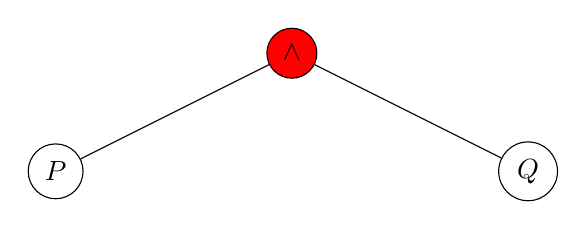
\begin{tikzpicture}[level/.style={sibling distance=60mm/#1}]
            \node [circle,draw,fill=red] (z){$\land$}
                child {node [circle,draw] (a) {$P$}}
                child {node [circle,draw] (b) {$Q$}};
        \end{tikzpicture}
        \caption{Binary node (red) binding variables}
        \label{fig:binaryNode}
    \end{figure}
    \item \emph{Unary} nodes representing unary operations that only have a single outgoing connection
    \begin{figure}[H]
        \centering
        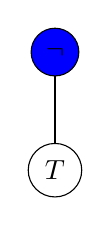
\begin{tikzpicture}[level/.style={sibling distance=60mm/#1}]
            \node [circle,draw,fill=blue] (z){$\neg$}
                child {node [circle,draw] (b) {$T$}};
        \end{tikzpicture}
        \caption{Unary node (blue) with a single constant child node}
        \label{fig:unaryNode}
    \end{figure}
    \item \emph{Leaf}-nodes representing a variable or a constant, which have no outgoing connections
    \begin{figure}[H]
        \centering
        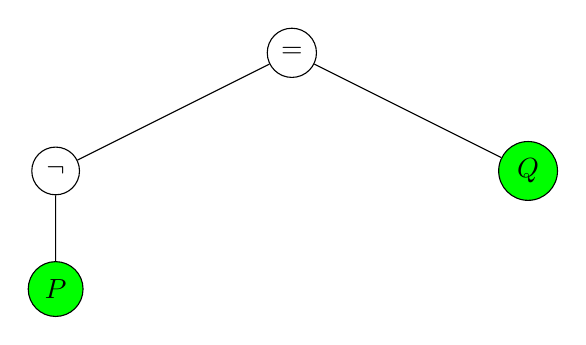
\begin{tikzpicture}[level/.style={sibling distance=60mm/#1}]
            \node [circle,draw] (z){$=$}
                child {node [circle,draw] (a) {$\neg$}
                    child {node [circle, draw, fill=green] (c) {$P$}}
                    }
                child {node [circle,draw, fill=green] (b) {$Q$}};
        \end{tikzpicture}
        \caption{Leaves (green) in an AST}
        \label{fig:leaves}
    \end{figure}
\end{itemize}

The components required to provide the conversion functionality can be structured in a similar fashion as the other converter components using the SOLID-principle. An abstract \emph{node converter} is introduced hiding the three different converter types to convert the three node types, which then again are split in two, to separate the conversion directions.

With the conversion infrastructure in place, it is now time to look for an algorithm that can handle the tree traversal during the conversion. In the case of ASTs, there are two approaches of traversal: The \emph{bottom-up} approach, where the tree analysis begins at the leaves, working its way up towards the root, and the \emph{top-down} approach, starting at the root, ending at the leaves.

From a performance point of view, algorithms using the bottom-up approach are have a better performance as they only need to traverse each node once. In top-down approaches the algorithms need to back-trace their steps to a previous node, as branches in the tree may split, forcing them to prioritise one node over the other.

In order to obtain the performance benefit fro the bottom-up approach it is required that the leaves of the tree can be accessed directly, and that children (lower-level nodes) have a reference to their parent (higher-level nodes). Both in SBML-qual and ERODE, the only directly accessible node is the root of the AST. This causes any bottom-up algorithm to lose its performance benefit, as they new require a data structure transformation to make the leaves of the AST accessible.

Due to the fact, that there is no performance loss and no additional structural transformation required, it is both viable and also much simpler to use a top-down approach. A suitable algorithm for such a tree traversal is a \emph{DFS} (depth-first-search). The algorithm will traverse down the branches of the tree, analyzing each node in the search for leaves. Since leaves have no children and can be converted instantly. In case a node is not a leaf, it will advance to its leftmost child, that has not been converted and analyze it. Once the algorithm finds a leaf, it will convert the leaf and backtrack converting each node on the way, that no longer requires other nodes to be converted first. The nodes are all nodes, whose children already have been converted.

If the algorithm finds a node that requires an additional child to be converted, it will initiate a recursive search in the sub-tree, that has the child as a root. Once again, the algorithm will search for a leaf that can be converted and repeat the backtracking once it has been converted.
Eventually, all nodes will be converted, since all ASTs have leaves and the conversion of leaves eventually make other nodes convertible. The now convertible nodes, no longer have children requiring conversion, the conversion process can be repeated until all nodes have been converted.

Since all nodes in the tree require some constant amount of work to be converted and all nodes in the tree must be converted, the algorithm is tightly bounded by $\Theta{(n)}$, where $n$ is the amount of nodes in the tree. The fact, that this algorithm is tightly bounded by the amount of nodes in the graph, means that both the worst-case and the best-case scenarios for the execution of the algorithm have a linear time complexity.
\subsection{Showcase depth-first-search}
\begin{figure}[H]
    \centering
    \begin{subfigure}[b]{0.3\textwidth}
        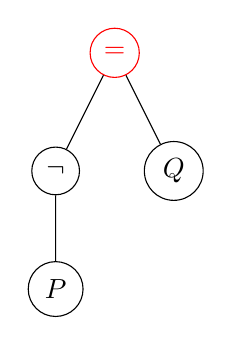
\begin{tikzpicture}
            \node [circle,draw, color=red] (z){$=$}
                child {node [circle,draw] (a) {$\neg$}
                    child {node [circle, draw] (c) {$P$}}
                    }
                child {node [circle,draw] (b) {$Q$}};
        \end{tikzpicture}
        \caption{(Analyze root}
    \end{subfigure}
    \begin{subfigure}[b]{0.3\textwidth}
        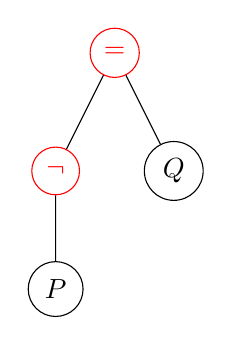
\begin{tikzpicture}
            \node [circle,draw, color=red] (z){$=$}
                child {node [circle,draw, color=red] (a) {$\neg$}
                    child {node [circle, draw] (c) {$P$}}
                    }
                child {node [circle,draw] (b) {$Q$}};
        \end{tikzpicture}
        \caption{Analyze left child}
    \end{subfigure}
    \begin{subfigure}[b]{0.3\textwidth}
        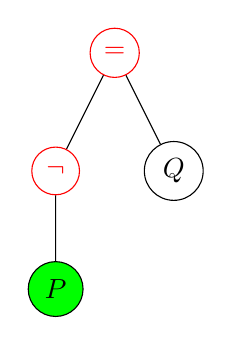
\begin{tikzpicture}
            \node [circle,draw, color=red] (z){$=$}
                child {node [circle,draw, color=red] (a) {$\neg$}
                    child {node [circle, draw, fill=green] (c) {$P$}}
                    }
                child {node [circle,draw] (b) {$Q$}};
        \end{tikzpicture}
        \caption{Convert $P$}
    \end{subfigure}
    \begin{subfigure}[b]{0.3\textwidth}
        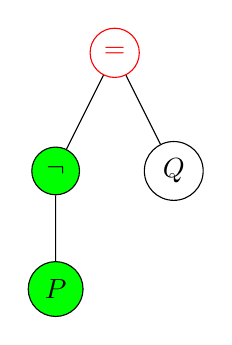
\begin{tikzpicture}
            \node [circle,draw, color=red] (z){$=$}
                child {node [circle,draw, fill=green] (a) {$\neg$}
                    child {node [circle, draw, fill=green] (c) {$P$}}
                    }
                child {node [circle,draw] (b) {$Q$}};
        \end{tikzpicture}
        \caption{Convert $\neg$}
    \end{subfigure}
    \begin{subfigure}[b]{0.3\textwidth}
        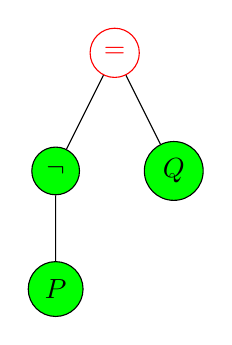
\begin{tikzpicture}
            \node [circle,draw, color=red] (z){$=$}
                child {node [circle,draw, fill=green] (a) {$\neg$}
                    child {node [circle, draw, fill=green] (c) {$P$}}
                    }
                child {node [circle,draw, fill=green] (b) {$Q$}};
        \end{tikzpicture}
        \caption{Convert $Q$}
    \end{subfigure}
    \begin{subfigure}[b]{0.3\textwidth}
        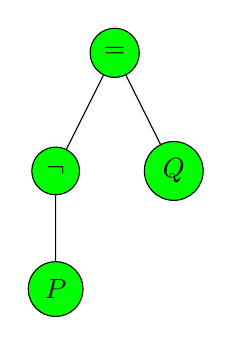
\begin{tikzpicture}
            \node [circle,draw, fill=green] (z){$=$}
                child {node [circle,draw, fill=green] (a) {$\neg$}
                    child {node [circle, draw, fill=green] (c) {$P$}}
                    }
                child {node [circle,draw, fill=green] (b) {$Q$}};
        \end{tikzpicture}
        \caption{Convert $=$}
    \end{subfigure}
\end{figure}